\section{Estimativas de usuários}

Esta seção tem como objetivo traçar uma estimativa dos possíveis usuários da plataforma desenvolvida, com o intuito de fornecer embasamento aos cálculos para realizar as previsões financeiras.

\subsection{Aplicações com público-alvo semelhantes}\label{subsec::publico-alvo_semelhante}

Neste tópico, serão analisadas as plataformas que possuem um público-alvo semelhante ao da \textit{GameLocker}. O objetivo da análise é alcançar um valor equilibrado para a assinatura \textit{premium} do sistema e realizar uma estimativa geral dos usuários que podem ser alcançados, levando em consideração a proporção de uma plataforma recém-lançada.

\subsubsection{Discord}

A plataforma \textit{\gls{Discord}} engloba chamadas de voz, mensagens escritas e uma gama variada de recursos para seus usuários. Conforme citado por Ash Turner \cite{discord_users}, aproximadamente 70\% dos usuários da plataforma a utilizam para jogar \textit{videogame} e outras atividades, como grupos de estudos. Essa informação leva à conclusão de que o público-alvo desse sistema se assemelha ao da \textit{GameLocker}.

De acordo com informações disponíveis no site oficial do \textit{\gls{Discord}} (Disponível em: \url{https://discord.com/nitro}), a plataforma oferece uma opção de assinatura mensal ao custo de \textit{R\$ 25,00}. Essa assinatura proporciona aos utilizadores a expansão da capacidade de \textit{uploads} de arquivos, uma personalização mais profunda de perfis, bem como a capacidade de transmitir vídeos em alta definição (HD), entre outros benefícios de significativa relevância.

\subsubsection{Twitch}

A \textit{\gls{Twitch}}, atualmente, desempenha um papel de destaque como uma das mais renomadas plataformas de transmissão em tempo real global. Conforme apontado pela VentureBeat \cite{twitch_categories}, nove das dez categorias mais assistidas na \textit{\gls{Twitch}} estão relacionadas a jogos eletrônicos, mantendo-se constantemente em evidência e atraindo diariamente centenas de milhares de espectadores. Essa dinâmica a torna um espaço amplamente explorado pelo público-alvo que este projeto busca alcançar.

De acordo com informações disponíveis em seu site oficial \url{https://www.twitch.tv}, a plataforma oferece uma opção de assinatura mensal com um custo de \textit{R\$ 26,99}. Através dessa assinatura, os usuários podem desfrutar da visualização de conteúdo livre de anúncios indesejados e têm acesso a um conjunto diversificado de recursos destinados à personalização de seus perfis. Isso inclui a utilização de \textit{emotes} personalizados, a variação de paletas de cores e a obtenção de distintivos especiais, contribuindo assim para uma experiência mais envolvente e individualizada.

\subsubsection{Estratégias de Utilização}

Este tópico visa investigar e analisar as estratégias que transformaram o \textit{\gls{Discord}} e o \textit{\gls{Twitch}} em líderes na arena da comunicação online, transcendo as suas origens como plataformas voltadas para jogos. Além disso, serão apresentadas estatísticas relacionadas ao uso e à receita dessas plataformas.

\subsubsubsection{Plano de Aplicação}

O \textit{\gls{Discord}}, desde a sua introdução em 2015, tem percorrido uma notável trajetória de evolução e adaptação, culminando na redefinição de sua imagem inicial, que estava originalmente vinculada a uma plataforma exclusivamente voltada para jogos.

\begin{itemize}
    \item \textbf{Diversificação de Servidores}: Servidores dedicados a jogos, permitindo que os jogadores se reunissem em um ambiente específico para cada jogo;
    \item \textbf{Expansão para Além dos Jogos}: Embora tenha começado como uma plataforma de jogos, o \textit{\gls{Discord}} expandiu sua base de usuários para incluir não jogadores, competindo com ferramentas de comunicação empresarial como \textit{Slack} e \textit{Microsoft Teams};
    \item \textbf{Combate à Controvérsia}: O \textit{\gls{Discord}} enfrentou desafios, incluindo a controvérsia em torno do uso de servidores privados por grupos extremistas. A empresa implementou ferramentas de moderação e verificação para lidar com esses problemas, destacando seu compromisso com a segurança e responsabilidade.
\end{itemize}

A \textit{\gls{Twitch}}, uma plataforma líder de comunicação, tem expandido significativamente seu escopo muito além de sua imagem inicial, que estava predominantemente associada à transmissão de jogos.

\begin{itemize}
    \item \textbf{Diversificação de Conteúdo}: Embora o \textit{\gls{Twitch}} seja amplamente associado à transmissão de jogos, a plataforma diversificou seu conteúdo ao longo do tempo. Além das transmissões de jogos, os criadores agora utilizam o \textit{Just Chatting} e outras categorias para transmitir uma variedade de conteúdos, como shows ao vivo, música e arte;
    \item \textbf{Parcerias e Integrações}: Estabelecer parcerias estratégicas com empresas e criadores de conteúdo, o que ajudou a atrair um público diversificado. Além disso, integrações com plataformas como \textit{\gls{Amazon Prime}} e eventos como o \textit{TwitchCon} fortaleceram a presença da plataforma;
    \item \textbf{Monetização para Criadores}: Introduzir maneiras inovadoras de monetização para criadores, como assinaturas de canais, doações e anúncios. Essas estratégias tornaram possível que criadores ganhassem renda significativa transmitindo seu conteúdo na plataforma.
\end{itemize}

\subsubsubsection{Estatísticas de Uso e Receita}

A \textit{\gls{Twitch}} registra 140 milhões de usuários ativos mensais, demonstrando sua extensa popularidade. Essa estatística por si só destaca a importância da plataforma no cenário de entretenimento online. Conforme apontado pela Backlink \cite{twitch_growth_statistics} e descrito na Figura \ref{crescimentoUsoTwitch}.

\begin{figure}[H]
    \center
	\caption{\label{fig_sge20}Crescimento do Uso da Twitch}
    \label{crescimentoUsoTwitch}
    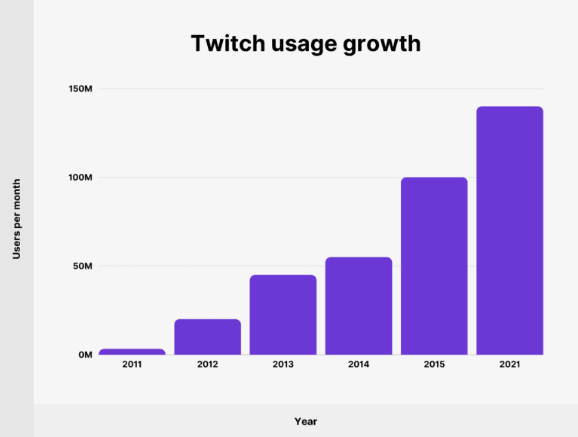
\includegraphics[scale=0.85]{imagens/viabilidadeFinanceira/CrescimentoTwitch.png}
	\fonte{\cite{twitch_growth_statistics}}
\end{figure}

Com 7,4 milhões de \textit{streamers} criando conteúdo a cada mês e um total de 9,2 milhões de \textit{streamers} ativos, fica claro que a comunidade de criadores desempenha um papel fundamental na expansão do \textit{\gls{Twitch}}. Os espectadores do \textit{\gls{Twitch}} assistem coletivamente a uma incrível quantidade de conteúdo, totalizando 1,14 trilhão de minutos assistidos, equivalentes a 1,86 bilhão de horas mensais.

Em termos de receita anual de publicidade, o \textit{\gls{Twitch}} alcançou a marca de US\$ 231,8 milhões, representando mais que o dobro dos US\$ 102,5 milhões registrados em 2017. Além da publicidade, outra fonte significativa de receita para o \textit{\gls{Twitch}} é o sistema de assinaturas. No entanto, a avaliação precisa dessa receita é desafiadora, uma vez que as assinaturas \textit{premium} do \textit{\gls{Amazon Prime}} incluem automaticamente a assinatura \textit{premium} do \textit{\gls{Twitch}}. Estimativas indicam que a receita anual total do \textit{\gls{Twitch}} gira em torno de US\$ 1,54 bilhão.

No que tange à base de usuários, o \textit{\gls{Discord}} ostenta números notáveis, com uma marca impressionante de 140 milhões de usuários ativos mensais, conforme demonstra a Figura \ref{usuariosMensaisDiscord}. Mais notável ainda é o fato de que essa base dobrou no último ano, o que atesta um crescimento substancial e sustentado ao longo do tempo. 

\begin{figure}[H]
    \center
	\caption{\label{fig_sge20}Usuários ativos mensais do Discord}
    \label{usuariosMensaisDiscord}
    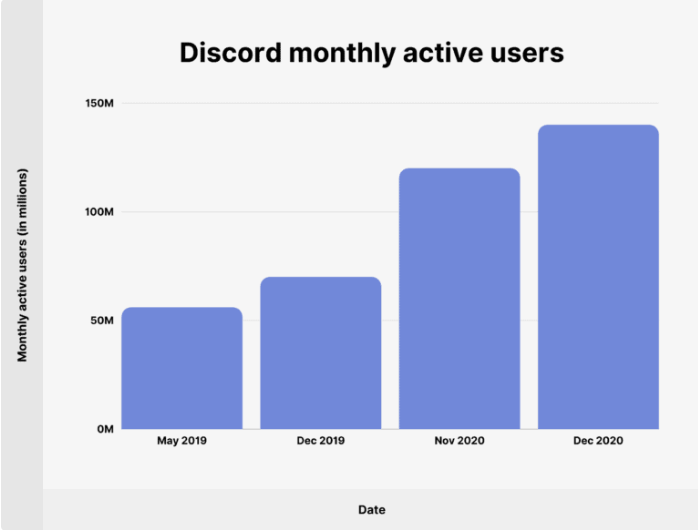
\includegraphics[scale=0.7]{imagens/viabilidadeFinanceira/DiscordActiveUsers.png}
	\fonte{\cite{discord_active_users}}
\end{figure}

No âmbito dos investimentos, o \textit{\gls{Discord}} angariou uma expressiva quantia de financiamento, totalizando US\$ 483,8 milhões. Além disso, o \textit{\gls{Discord}} demonstra sua capacidade de monetização ao gerar uma receita anual considerável, totalizando US\$ 130 milhões. Com uma valoração atual de US\$ 7 bilhões e uma rede de cerca de 13,5 milhões de servidores ativos por semana, o \textit{\gls{Discord}} emerge como um protagonista fundamental no cenário das interações online, consolidando-se como uma das principais plataformas de comunicação no mundo.

\subsection{Análise e Projeção}

Para estimar o crescimento de usuários do projeto, foi adotada como abordagem de análise uma curva normal de crescimento. Estabelecemos como meta de projeção um incremento de 1\% no número de usuários ativos em relação às duas plataformas mencionadas, ao término dos primeiros 12 meses.

A projeção de um aumento de 1\% ao longo do período de 12 meses resultaria em um total de 30.000 usuários ativos na plataforma. Ressalta-se a relevância deste crescimento gradual, o qual segue uma trajetória ascendente que se alinha com as tendências observadas na \textit{\gls{Twitch}} e no \textit{\gls{Discord}}. Cabe destacar que, embora o projeto esteja em estágio inicial e não disponha da mesma base de usuários das plataformas mencionadas, a tendência de crescimento sustentado é promissora.

Com base nas informações disponíveis sobre a \textit{\gls{Twitch}} e o \textit{\gls{Discord}}, é plenamente justificável projetar um aumento gradual para o presente projeto. As referidas plataformas representam notáveis exemplos de sucesso no âmbito do entretenimento online e da comunicação, o que reflete a crescente demanda por tais serviços. Nesse contexto, a estimativa de crescimento de usuários apresentada neste estudo está fundamentada em bases sólidas e aponta para um considerável potencial.